%%%%%%%%%%%%%%%%%%%%%%%%%%% asme2ej.tex %%%%%%%%%%%%%%%%%%%%%%%%%%%%%%%
% Template for producing ASME-format journal articles using LaTeX    %
% Written by   Harry H. Cheng, Professor and Director                %
%              Integration Engineering Laboratory                    %
%              Department of Mechanical and Aeronautical Engineering %
%              University of California                              %
%              Davis, CA 95616                                       %
%              Tel: (530) 752-5020 (office)                          %
%                   (530) 752-1028 (lab)                             %
%              Fax: (530) 752-4158                                   %
%              Email: hhcheng@ucdavis.edu                            %
%              WWW:   http://iel.ucdavis.edu/people/cheng.html       %
%              May 7, 1994                                           %
% Modified: February 16, 2001 by Harry H. Cheng                      %
% Modified: January  01, 2003 by Geoffrey R. Shiflett                %
% Butchered: October 15, 2014 by John Karasinski                     %
% Use at your own risk, send complaints to /dev/null                 %
%%%%%%%%%%%%%%%%%%%%%%%%%%%%%%%%%%%%%%%%%%%%%%%%%%%%%%%%%%%%%%%%%%%%%%

%%% use twocolumn and 10pt options with the asme2ej format
\documentclass[twocolumn,10pt]{asme2ej}

\usepackage{epsfig} %% for loading postscript figures
\usepackage{amsmath}
\usepackage{graphicx}
\usepackage{grffile}
\usepackage{pdfpages}
\usepackage{algpseudocode}

% Default fixed font does not support bold face
\DeclareFixedFont{\ttb}{T1}{txtt}{bx}{n}{12} % for bold
\DeclareFixedFont{\ttm}{T1}{txtt}{m}{n}{12}  % for normal

% Custom colors
\usepackage{color}
\usepackage{listings}

\definecolor{mygreen}{rgb}{0,0.6,0}
\definecolor{mygray}{rgb}{0.5,0.5,0.5}
\definecolor{mymauve}{rgb}{0.58,0,0.82}

\lstset{ %
  backgroundcolor=\color{white},   % choose the background color; you must add \usepackage{color} or \usepackage{xcolor}
  basicstyle=\ttfamily\footnotesize, % the size of the fonts that are used for the code
  breakatwhitespace=false,         % sets if automatic breaks should only happen at whitespace
  % breaklines=true,                 % sets automatic line breaking
  captionpos=b,                    % sets the caption-position to bottom
  commentstyle=\color{mygreen},    % comment style
  deletekeywords={...},            % if you want to delete keywords from the given language
  escapeinside={\%*}{*)},          % if you want to add LaTeX within your code
  extendedchars=true,              % lets you use non-ASCII characters; for 8-bits encodings only, does not work with UTF-8
  frame=single,                    % adds a frame around the code
  keepspaces=true,                 % keeps spaces in text, useful for keeping indentation of code (possibly needs columns=flexible)
  columns=flexible,
  keywordstyle=\color{blue},       % keyword style
  language=Python,                 % the language of the code
  morekeywords={*,...},            % if you want to add more keywords to the set
  numbers=left,                    % where to put the line-numbers; possible values are (none, left, right)
  numbersep=5pt,                   % how far the line-numbers are from the code
  numberstyle=\tiny\color{mygray}, % the style that is used for the line-numbers
  rulecolor=\color{black},         % if not set, the frame-color may be changed on line-breaks within not-black text (e.g. comments (green here))
  showspaces=false,                % show spaces everywhere adding particular underscores; it overrides 'showstringspaces'
  showstringspaces=false,          % underline spaces within strings only
  showtabs=false,                  % show tabs within strings adding particular underscores
  stepnumber=1,                    % the step between two line-numbers. If it's 1, each line will be numbered
  stringstyle=\color{mymauve},     % string literal style
  tabsize=4,                       % sets default tabsize to 2 spaces
}

\title{Case Study \# 3: Structural Analysis: Perforated Plate in Tension}

\author{John Karasinski
    \affiliation{
  Graduate Student Researcher\\
  Center for Human/Robotics/Vehicle Integration and Performance\\
  Department of Mechanical and Aerospace Engineering\\
  University of California\\
  Davis, California 95616\\
    Email: karasinski@ucdavis.edu
    }
}

\begin{document}
\maketitle

%%%%%%%%%%%%%%%%%%%%%%%%%%%%%%%%%%%%%%%%%%%%%%%%%%%%%%%%%%%%%%%%%%%%%%
\section{Problem Description}
This case study involves a linear-elastic, steady-state stress analysis on a square plate with a circular hole at its center. The plate dimensions are: side length $x = 4$m and radius $R = 0.5$m. It is loaded with a uniform traction of $\sigma = 10$kPa over its left and right faces as can be seen in Figure~\ref{geometry}.

A mesh sensitivity study is performd for a plate with side length $x = 4$m, and an effect of the plate length study is performed for plates of length $x = 3$m, 4m, 5m, and 100m. The stress normal to the vertical plane of symmetry is calculated for each case, and the results are compared to the analytical solution:
\begin{equation}
(\sigma_{xx})_{x=0} \left\{ \begin{array}{lll}
        \mbox{$\sigma(1+\frac{R^2}{2y^2}+\frac{3R^4}{2y^4}) $} & \mbox{for } &|y| \geq R \\
        \mbox{$0$} & \mbox{for } &|y| < R \end{array}. \right.
\label{vertical_stress}
\end{equation}

Similarly, the stress normal to the horizontal plane of symmetry can also be computed and compared to the analytical solution:
\begin{equation}
(\sigma_{yy})_{y=0} \left\{ \begin{array}{lll}
        \mbox{$\sigma(\frac{R^2}{2x^2}-\frac{3R^4}{2x^4}) $} & \mbox{for } &|x| \geq R \\
        \mbox{$0$} & \mbox{for } &|x| < R \end{array}. \right.
\label{horizontal_stress}
\end{equation}

A Python script was created to automatically generate the configuration files, calculate the resulting steady-state stress through the plate using OpenFOAM \cite{jasak2007openfoam}, and plot the results for both the sensitivity and plate length studies. This script is included in the Appendix.

\begin{figure}[t]
\begin{center}
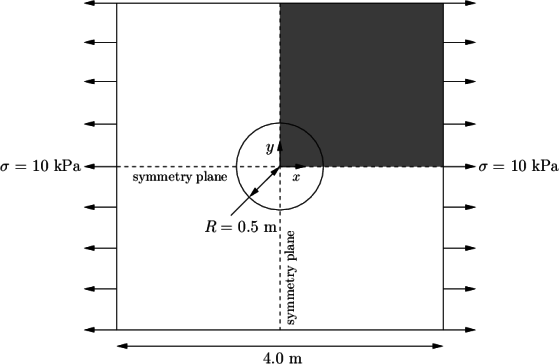
\includegraphics[width=0.45\textwidth]{figure/user144x.png}
\caption{Geometry of the plate with a hole \cite{ctfm_1}}
\label{geometry}
\end{center}
\end{figure}

%%%%%%%%%%%%%%%%%%%%%%%%%%%%%%%%%%%%%%%%%%%%%%%%%%%%%%%%%%%%%%%%%%%%%%
\section{Numerical Solution Approach}
 Two symmetry planes can be identified for this geometry and therefore the solution domain need only cover a quarter of the geometry, shown by the shaded area in Figure~\ref{geometry}. The quarter plate is then broken into five blocks of varying sizes, as can be seen in Figure~\ref{blocks}. These blocks have a multiple of the characteristic number of points, $n$, in the $x_i$ and $y_i$ directions. Blocks 0 and 1 consist of $n$ by $n$ points, block 2 consists of $2n$ by $n$ points, block 3 consists of $2n$ by $2n$ points, and block 4 consists of $n$ by $2n$ points. The mesh is generated with OpenFOAM's `blockMesh' command, and the resulting mesh for $n = 10$ can be seen in Figure~\ref{mesh}.

 The mesh sensitivity study looks at meshes resulting from $n = 10, 100, $ and $1000$ on a plate width of $x = 4$m. The effect of plate length study looks at plate lengths of $x = 3$m, 4m, 5m, and 100m with a mesh of $n = 10$. Once the meshes have been generated, OpenFOAM's `solidDisplacementFoam' solver runs the simulation, and $\sigma_{xx}$ is calculated and sampled by the OpenFOAM commands `foamCalc components sigma' and `sample'. The `solidDisplacementFoam' solver is a transient segregated finite-volume solver for linear-elastic, small-strain deformation of a solid body, and is well suited to solve this problem.
\begin{figure}[thb]
\begin{center}
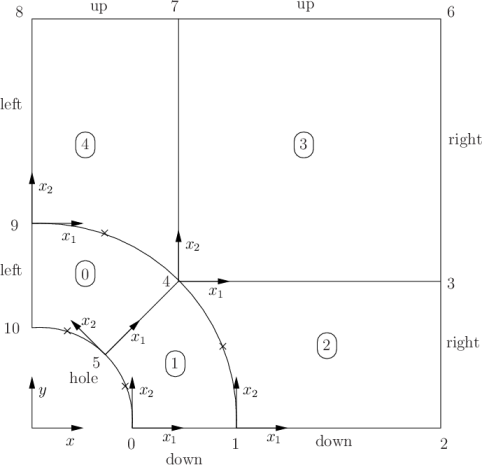
\includegraphics[width=0.45\textwidth]{figure/user149x.png}
\caption{Block structure of the mesh for the plate with a hole \cite{ctfm_1}}
\label{blocks}
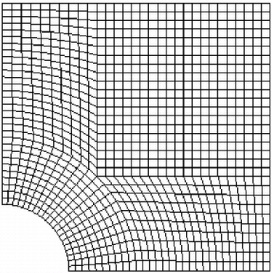
\includegraphics[width=0.45\textwidth]{figure/user152x.png}
\caption{Mesh of the hole in a plate problem with $n = 10$ \cite{ctfm_1}}
\label{mesh}
\end{center}
\end{figure}

%%%%%%%%%%%%%%%%%%%%%%%%%%%%%%%%%%%%%%%%%%%%%%%%%%%%%%%%%%%%%%%%%%%%%%
\section{Results Discussion}
The computational result for normal stress along the vertical and horizontal symmetries can be compared to the analyticals result above, Equations~\ref{vertical_stress} and~\ref{horizontal_stress}. The Root Mean Square error,
\begin{equation}
\mbox{RMSE} = \sqrt{\frac{1}{N}\sum\limits_{i=1}^N[\sigma_i - \sigma^*_i]^2},
\end{equation}
and the Normalized Root Mean Square error,
\begin{equation}
\mbox{NRMS} = \dfrac{RMSE}{max(\sigma^*)-min(\sigma^*)},
\end{equation}
can be calculated. Here $\sigma_i$ is the computational result for the the stress for each point along the boundary, $\sigma^*_i$ is the analytical solution, and $N$ is the number of points along the boundary. The NRMS for each case is expressed as a percentage, where lower values indicate a result closer to the analytic solution. For the remainder of this paper $NRMS_{xx}$ will note the NRMS error along the vertical plane of symmetry, while $NRMS_{yy}$ will note the NRMS error along the horizontal plane of symmetry.

\subsection{Selected key results for the base case}
The base case described in the OpenFOAM tutorial involves a plate of width $x = 4$ with a mesh resulting from $n = 10$ \cite{ctfm_1}. The NRMS from the analytical solution for this case is approximately 9.41\% for the vertical symmetry, and 18.36\% for the horizontal symmetry. The results for the normal stress along the symmetries and their deviation from the analytical solution for this case can be seen in Figure~\ref{base_study}.

A quick look at the error plots suggest that the stress along the vertical symmetry is overestimated, while the stress along the horizontal symmetry is underestimated. These results suggest that a square plate with a relatively low number of cells can fairly accurately reproduce the analytical solution of an infinitely wide plate for the vertical symmetry, but fails to do well in estimating the stress along the horizontal symmetry. Increasing the mesh and the length of the plate could lead to results that closer approximate this analytic solution.

\begin{figure}[b]
\begin{center}
\includegraphics[width=0.5\textwidth]{../code/figures/result-x-[2][10].pdf}
\includegraphics[width=0.5\textwidth]{../code/figures/error-x-[2][10].pdf}
\includegraphics[width=0.5\textwidth]{../code/figures/result-y-[2][10].pdf}
\includegraphics[width=0.5\textwidth]{../code/figures/error-y-[2][10].pdf}
\caption{Results of base case}
\label{base_study}
\end{center}
\end{figure}

\subsection{Mesh sensitivity study}
The mesh sensitivity study looks at meshes resulting from $n = 10, 100, $ and $1000$ on a plate width of $x = 4$m.

\begin{table}[htb]
%\caption{Figure and table captions do not end with a period}
\begin{center}
\label{mesh_table}
\begin{tabular}{|r r | r r|}
\hline
$x (m)$ & $n$ & $NRMS_{xx}$ & $NRMS_{yy}$ \\
\hline
4 & 10   & 9.41\% & 18.36\% \\
4 & 100  & 9.72\% & 18.77\% \\
4 & 1000 & 9.01\% & 17.43\% \\
\hline
\end{tabular}
\caption{NRMS results from the numerical simulations for the mesh sensitivity study}
\end{center}
\end{table}

\subsection{Effect of the plate length study}
The effect of plate length study looks at plate lengths of $x = 3$m, 4m, 5m, and 100m with a mesh of $n = 100$.

\begin{table}[htb]
%\caption{Figure and table captions do not end with a period}
\begin{center}
\label{mesh_table}
\begin{tabular}{|r r | r r|}
\hline
$x (m)$ & $n$ & $NRMS_{xx}$ & $NRMS_{yy}$ \\
\hline
3   & 100 & 15.02\% & 29.17\% \\
4   & 100 &  9.71\% & 18.77\% \\
5   & 100 &  6.46\% &  9.43\% \\
100 & 100 &  4.24\% &  5.96\% \\
\hline
\end{tabular}
\caption{NRMS results from the numerical simulations for the effect of plate length study}
\end{center}
\end{table}


\begin{figure}[tb]
\begin{center}
\includegraphics[width=0.5\textwidth]{../code/figures/result-x-[2, 2, 2][10, 100, 1000].pdf}
\includegraphics[width=0.5\textwidth]{../code/figures/error-x-[2, 2, 2][10, 100, 1000].pdf}
\includegraphics[width=0.5\textwidth]{../code/figures/result-y-[2, 2, 2][10, 100, 1000].pdf}
\includegraphics[width=0.5\textwidth]{../code/figures/error-y-[2, 2, 2][10, 100, 1000].pdf}
\caption{Results of mesh sensitivity study}
\label{sensitivity_study}
\end{center}
\end{figure}
\begin{figure}[tb]
\begin{center}
\includegraphics[width=0.5\textwidth]{../code/figures/result-x-[1.5, 2, 2.5, 50][100, 100, 100, 100].pdf}
\includegraphics[width=0.5\textwidth]{../code/figures/error-x-[1.5, 2, 2.5, 50][100, 100, 100, 100].pdf}
\includegraphics[width=0.5\textwidth]{../code/figures/result-y-[1.5, 2, 2.5, 50][100, 100, 100, 100].pdf}
\includegraphics[width=0.5\textwidth]{../code/figures/error-y-[1.5, 2, 2.5, 50][100, 100, 100, 100].pdf}
\caption{Results of plate length study}
\label{length_study}
\end{center}
\end{figure}


%%%%%%%%%%%%%%%%%%%%%%%%%%%%%%%%%%%%%%%%%%%%%%%%%%%%%%%%%%%%%%%%%%%%%%
\section{Conclusion}

%%%%%%%%%%%%%%%%%%%%%%%%%%%%%%%%%%%%%%%%%%%%%%%%%%%%%%%%%%%%%%%%%%%%%%
\bibliographystyle{asmems4}
\bibliography{asme2e}

%%%%%%%%%%%%%%%%%%%%%%%%%%%%%%%%%%%%%%%%%%%%%%%%%%%%%%%%%%%%%%%%%%%%%%
\clearpage
\onecolumn
\appendix       %%% starting appendix
\section*{Appendix A: Python Code}

\lstinputlisting[language=Python]{../code/CaseStudy3.py}

%%%%%%%%%%%%%%%%%%%%%%%%%%%%%%%%%%%%%%%%%%%%%%%%%%%%%%%%%%%%%%%%%%%%%%
\end{document}
